\section{Theoretical Result}\label{sec:fc}
\begin{theorem}\label{th:main} Let $\sigma=\frac{\cscale}{\sqrt{w}}$ and $\bfc= d\cdot\sigma^{d-1} $ Under \Cref{assmp:main}, a $w\ra\infty$, for FC-DGN we have: 
\begin{align*}
\kv_{\Tdgn_0}(x,x') \ra \bfc \cdot\ip{ x,x'} \cdot \Pi_{l=1}^{d-1} \frac{\ip{G_l(x),G_l(x')}}w
\end{align*}
\end{theorem}
$\bullet$ \textbf{Role of Weights:}  The weights of the feature network that dictate the NPFs (and hence the NPK) are more critical than the NPV (as long as the NPV is chosen as per \Cref{assmp:main}). Thus, the primary role of the weights is to generate the gates, i.e., the NPFs/NPK. In particular, copying the weights of a pre-trained DNN onto the feature network and training the NPV from scratch recovers the test accuracy of original pre-trained DNN within $1\%$ (see \Cref{sec:exp}). 

$\bullet$ \textbf{Role of Activations:} The ReLU is a special activation, that is, it acts as a gate and the gates themselves are learnt. In particular, learnt gates achieve better test accuracy than random gate (see \Cref{sec:exp}). Also note that, \Cref{th:main} applies to any arbitrary gating, i.e., the $w\ra\infty$ is only binding on the value network, in the case of feature network with finite width, the gates can be \emph{repeated} infinite times to meet the $w\ra\infty$ condition. 

$\bullet$ \textbf{Width} is responsible for averaging (division by $w$) of the base kernels.

$\bullet$ \textbf{Depth} gives rise to a product of base kernels. 

$\bullet$ \textbf{Permutation Invariance:} The NPK is invariant if the layers (as masks) are permuted. This is because the $\Pi_{l=1}^{d-1} \frac{H^{\text{lyr}}_{l,\Tf_0}(x,x')}{w}$ is permutation invariant. We verify this experimentally (see \Cref{sec:exp}).

$\bullet$ \textbf{Constant Inputs:} Even if the input to the value network is set of a constant, i.e., even if $\langle x,x'\rangle$ is made constant, the gates still hold information in the from of $\Pi_{l=1}^{d-1} \frac{H^{\text{lyr}}_{l,\Tf_0}(x,x')}{w}$. We verify this experimentally (see \Cref{sec:exp}).
\begin{comment}
\subsection{Convolution with pooling}

\begin{theorem}\label{th:mainconv} Let $\sigcnn=\frac{\cscale}{\sqrt{w\wconv}}$ for the convolutional layers and $\sigfc=\frac{\cscale}{\sqrt{w}}$ for FC layers. Under \Cref{assmp:main}, as $w\ra\infty$, with  $\bcnn = \ \left(\dconv \sigcnn^{2(\dconv-1)}\sigfc^{2\dfc}+\dfc \sigcnn^{2\dconv}\sigfc^{2(\dfc-1)}\right)$ we have:
\begin{align*}
&\kv_{\Tdgn_0}&\ra&\quad \frac{\bcnn}{{\din}^2} \cdot \sum_{r=0}^{\din-1} \ip{x,rot(x',r)}_{\Lambda(\cdot, x,rot(x',r))},\,\,\text{(for global-average-pooling)}\\
&\kv_{\Tdgn_0}&\ra& \quad{\bcnn} \cdot \sum_{r=0}^{\din-1} \ip{x,rot(x',r)}_{\Lambda(\cdot, x,rot(x',r))},\,\,\text{(for global-max-pooling)}\\
\end{align*}
\end{theorem}


\subsection{Skip Connections: Sum of Product Kernel}\label{sec:res}
In this section, we show that in the presence of skip connections, NPK has a sum of product structure. To illustrate our case, we consider a ResNet with `$(b+2)$' blocks and `$b$' skip connections between the blocks (\Cref{fig:resnet}). Each block is a FC-DNN of depth `$\dblock$' and width `$w$'. The sum of product structure is due to the combinatorially many sub-FC-DNNs within this ResNet (see \Cref{def:subfcdnn} and \Cref{fig:subfcdnn}).

\FloatBarrier
\begin{figure}[h]
\begin{minipage}{0.5\columnwidth}
\resizebox{\columnwidth}{!}{
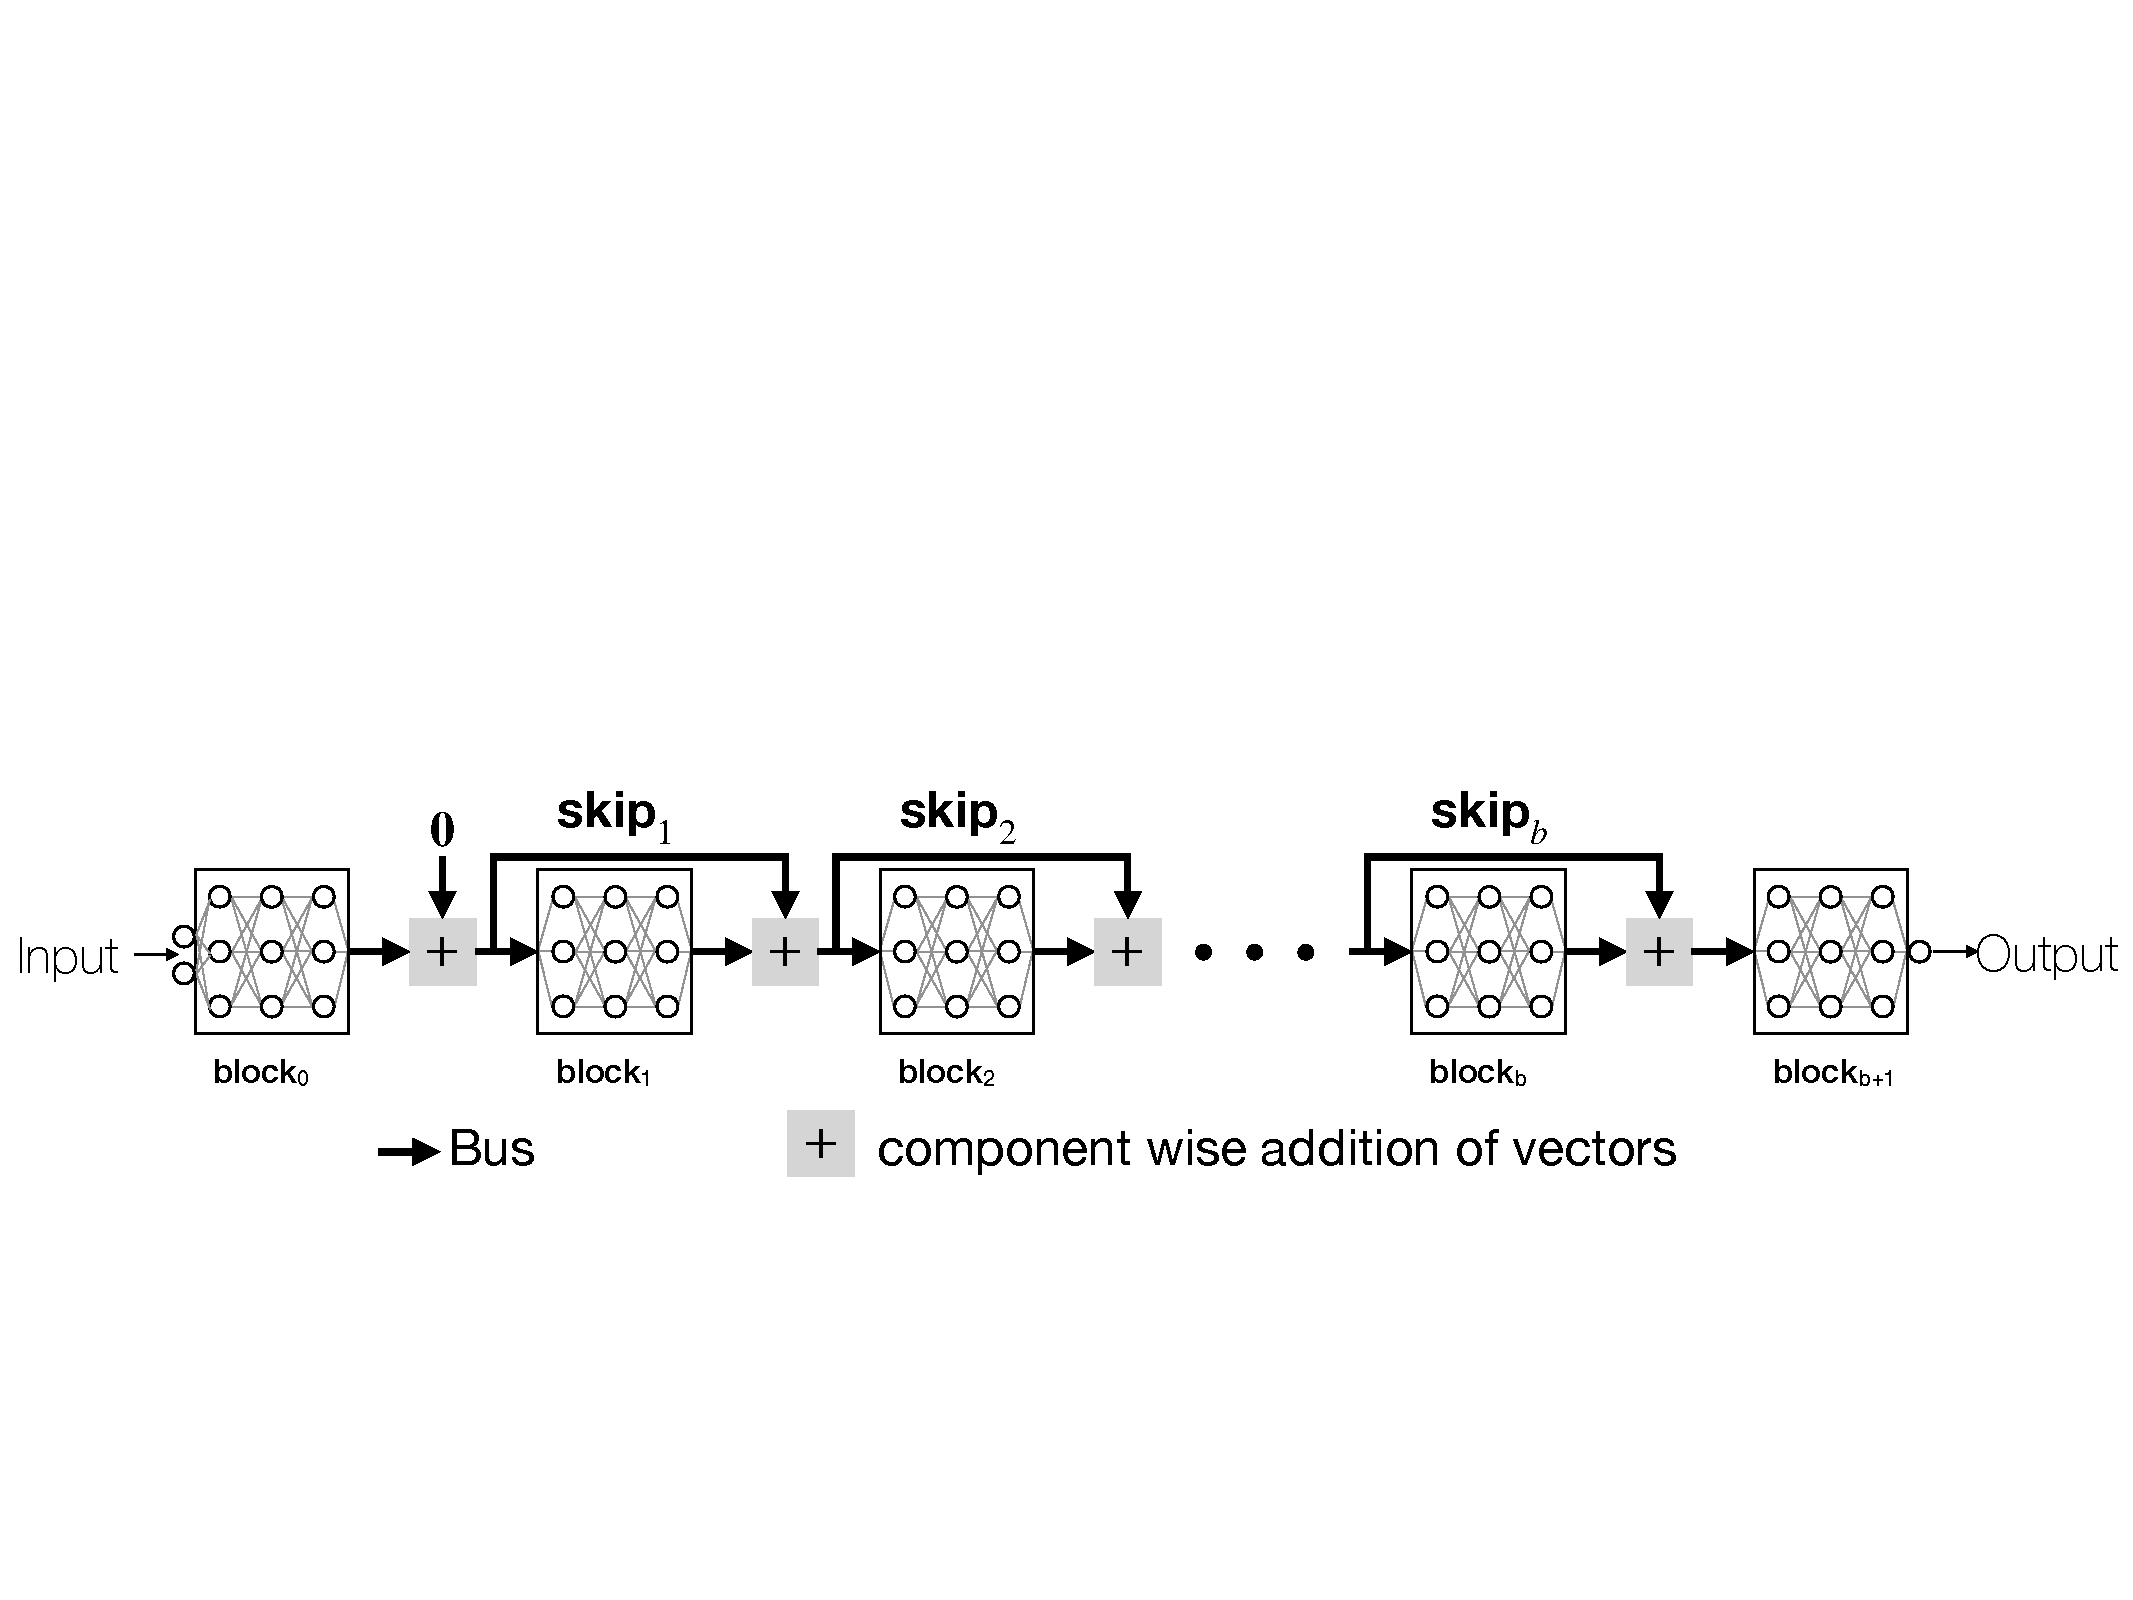
\includegraphics[scale=0.5]{figs/resnet.pdf}
}
\end{minipage}
\begin{minipage}{0.5\columnwidth}
\resizebox{\columnwidth}{!}{
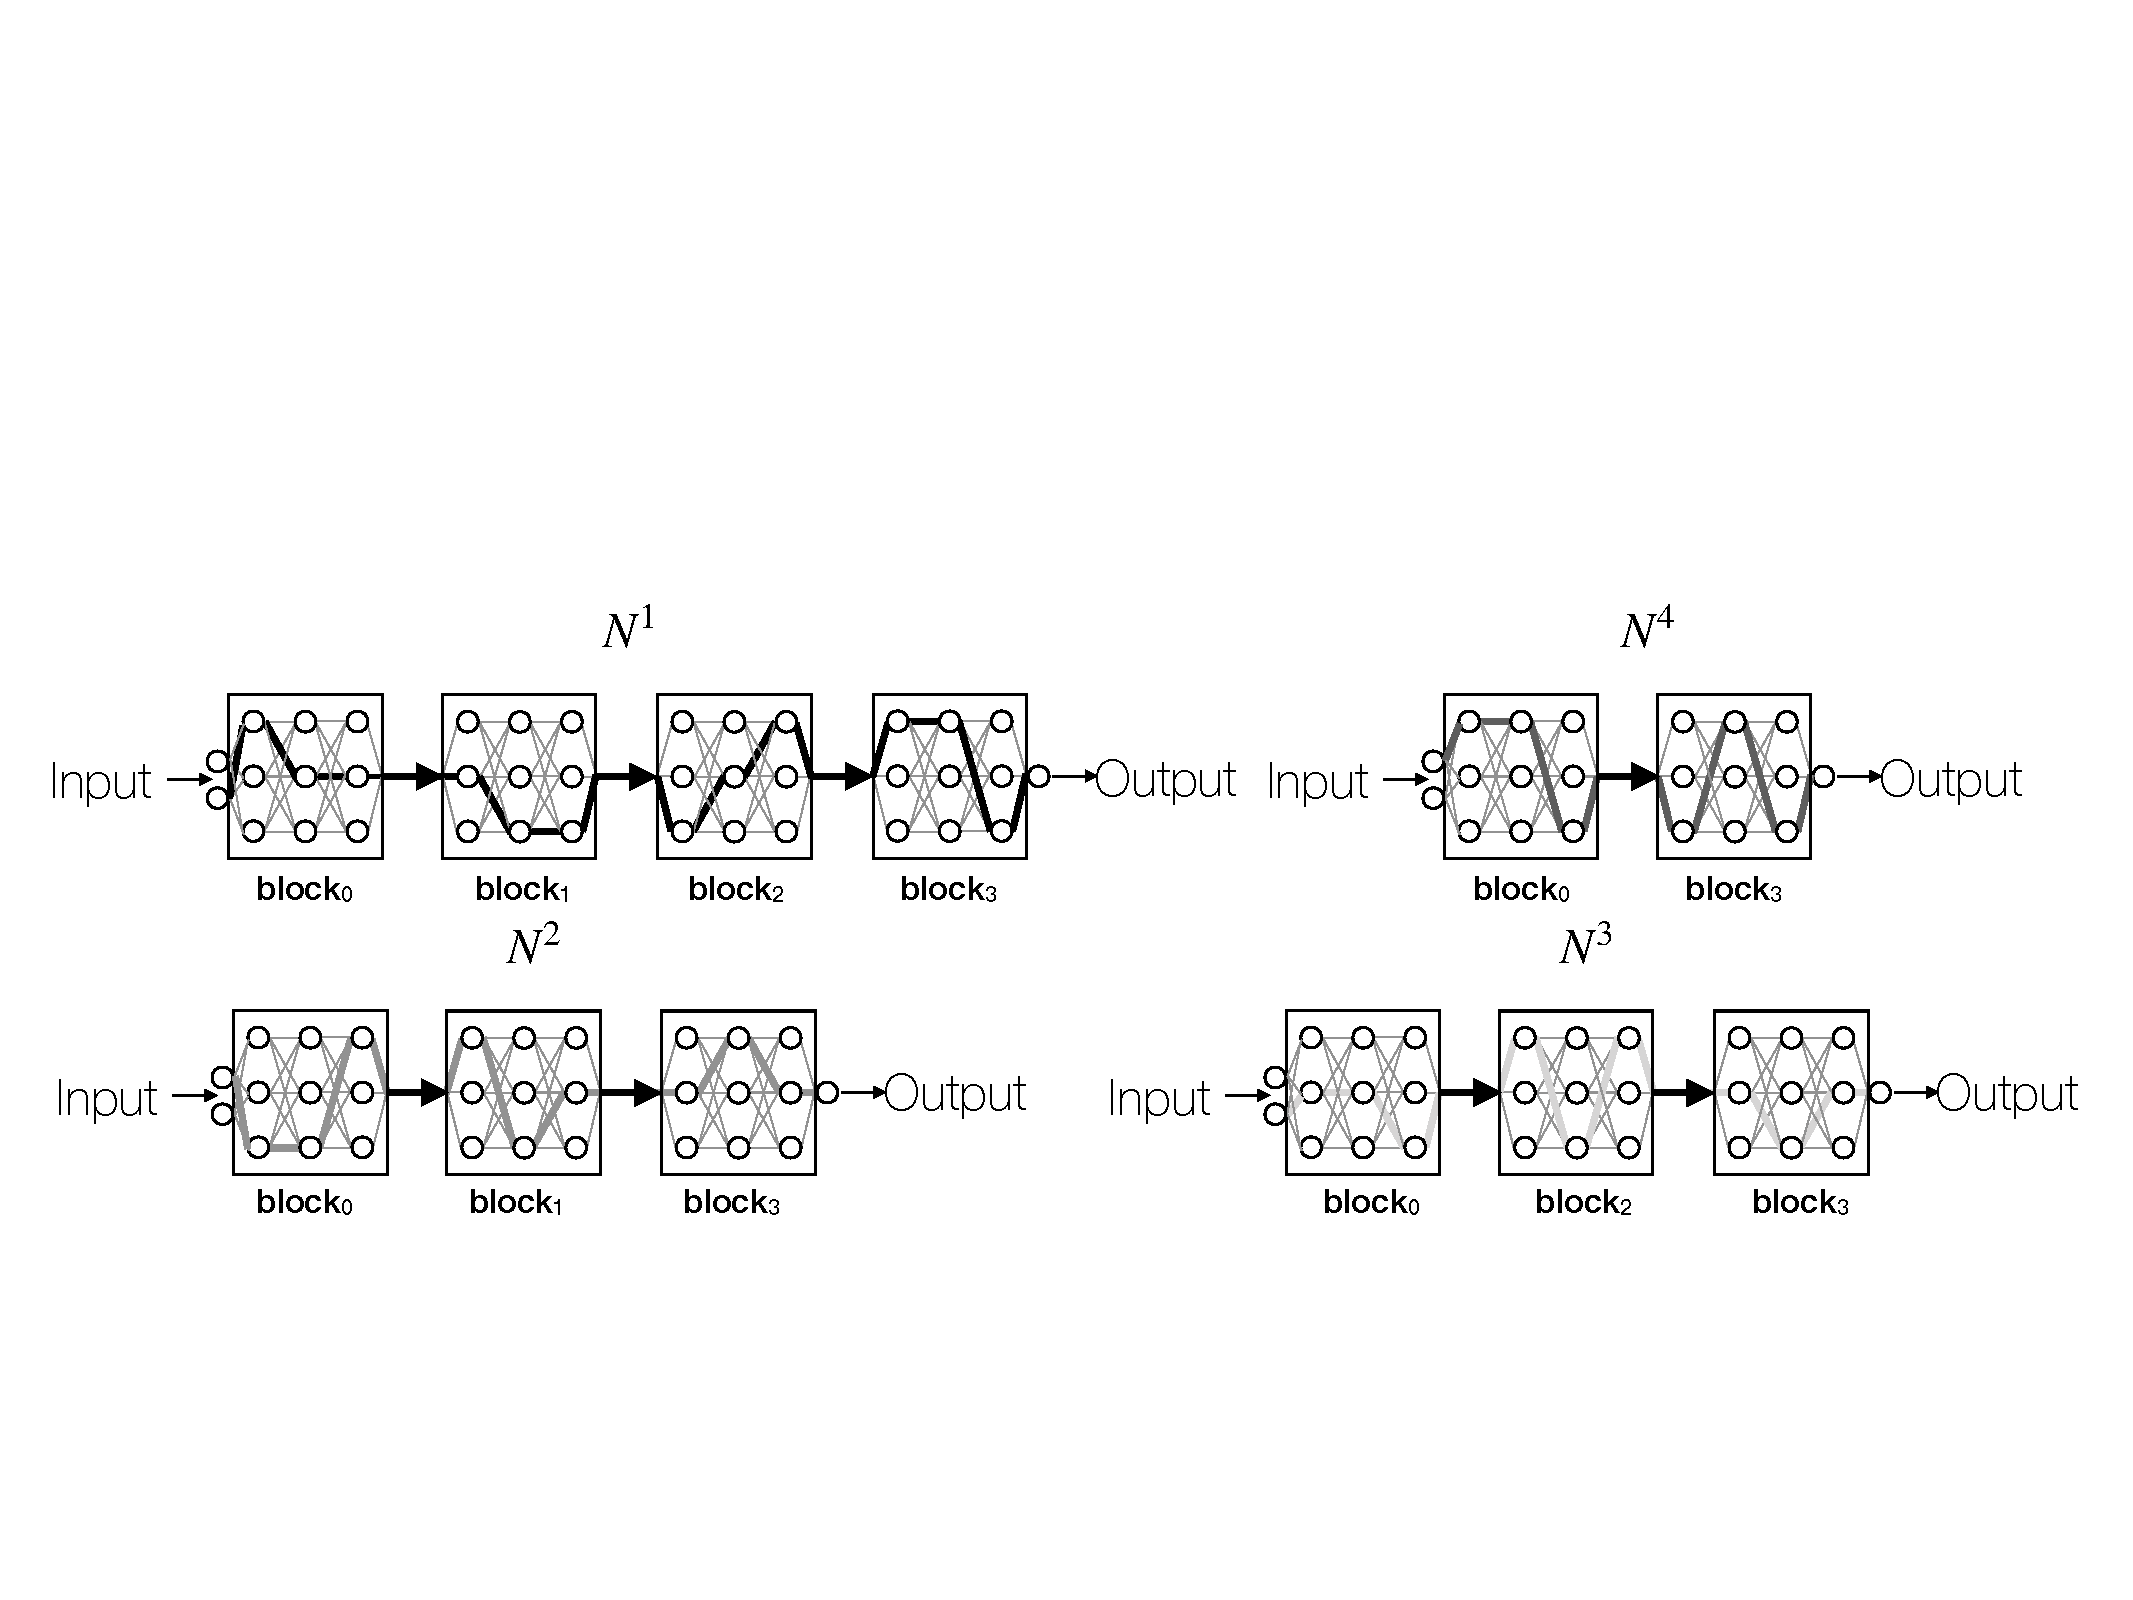
\includegraphics[scale=0.5]{figs/blocks.pdf}
}
\end{minipage}
\caption{\small{ResNet with $b$ skip connections and $(b+2)$ blocks.}}
\label{fig:resnet}
\end{figure}

\begin{definition}\label{def:subfcdnn}[Sub FC-DNNs]
Let $2^{[b]}$ denote the power set of $[b]$ and let $\J\in 2^{[b]}$ denote any subset of $[b]$. Define the`$\J^{th}$' sub-FC-DNN of the ResNet to be the fully connected network obtained by (i) ignoring/removing the skip connections $\text{skip}_j,\forall j\in \J$  and (ii) ignoring $\text{block}_{j},\forall j\notin \J$ (see \Cref{fig:resnet,fig:subfcdnn}).
\end{definition}
\begin{theorem}\label{th:mainres} Let $\sigma=\frac{\cscale}{\sqrt{w}}$. Under \Cref{assmp:main}, as $w\ra\infty$,  for $\bfc^{\J} = (|\J| +2)\cdot\dblock\cdot \sigma^{2\big( (|\J|+2)\dblock-1\big)}$,
\begin{align*}
\kv_{\Tdgn_0}\ra \sum_{\J\in 2^{[b]}}  \bfc^{\J} H^{\J}_{\Tf_0}
\end{align*}
\end{theorem}

\end{comment}